\chapter*{Fasi per il riconoscimento della posizione all'interno degli edifici}
L'identificazione della posizione all'interno di un edificio si svolge in 2 fasi:
\begin{enumerate}
	\item Scansione dell'ambiente
	\item Ricerca della posizione
\end{enumerate}

\section*{Scansione dell'ambiente}
Analisi statica dell'ambiente chiuso, nel quale il software raccogliera' le onde magnetiche per ogni intervallo di tempo, le classifichera' con una semplice label la quale rappresentera' la zona di appartenenza.\\
La scansione a sua volta composta da diverse sotto-fasi cio\`{e}:
\begin{enumerate}
	\item Raccoglimento dei dati
	\item Estrazione del magnitudo
	\item Raggruppamento
	\item Estrapolazione delle \textit{features}
\end{enumerate}
\newpage
\subsection*{Raccoglimento dei dati}
Innanzitutto esaminiamo la composizione dei dati che stiamo andando ad estrarre: si tratta di onde magnetiche quindi strutturate nel seguente modo:\\
\begin{center}
	$(x,\, y,\, z)$
\end{center}
I tre valori sono espressi in $ \mu T $ (micro Tesla), unita' di misura della densita' di un flusso magnetico. Ad ogni onda magnetica viene assegnata una \textit{label}: una stringa od un numero che identifica univocamente una parte dell'ambiente chiuso
\begin{figure}[H]
\centering
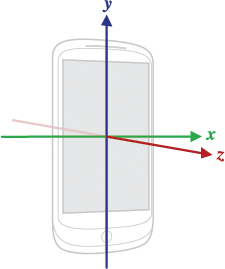
\includegraphics[width=0.20\linewidth]{./img/axis_magnetic_field.png}
\caption{Raffigurazione grafica delle onde raccolte}
\label{fig:axis_magnetic_field}
\end{figure}

\subsection*{Estrazione del magnitudo}
Per estrarre l'intensit\`{a} di ogni onda magnetica eseguiamo semplicemente la norma euclidea di un vettore:\\
\begin{center}
	$ \sqrt{x^2 + y^2 + z^2}$
\end{center}

\subsection*{Raggruppamento}
Le onde magnetiche con la stessa \textit{label} vengono raggruppate in \textit{fingerprints}, insiemi di dimensione prefissata. A livello logico, ogni \textit{fingerprint} cerca di identificare univocamente un punto all'interno di una zona, identificata con una \textit{label}. L'insieme di \textit{fingerprints} quindi, cerca di distinguere, tramite le caratteristiche dei campi elettromagnetici di ciascun punto, ogni \textit{label} dall'altra.

\subsection*{Estrapolazione delle \textit{features}}
Per ogni \textit{fingerprint}, l'estrazione delle \textit{features} consiste nell'estrazione di variabili statistiche. In questo specifico caso sono:
\begin{itemize}
	\item Media
	\item Varianza
	\item Deviazione standard
	\item Mediana
	\item Media troncata
	\item Coefficiente di variazione
	\item Massimo
	\item Minimo
	\item $ 1^{\circ}, 5^{\circ}, 95^{\circ}, 99^{\circ} $ percentile
	\item $ 1^{\circ}, 2^{\circ}, 3^{\circ} $ quartile
\end{itemize}



\section*{Ricerca della posizione}
Dopo aver scansionato l'ambiente questa fase viene eseguita dal cliente durante l'utilizzo dell'applicazione. La ricerca consiste nel creare sul momento una \textit{fingerprint} e poi, tramite un algoritmo di apprendimento automatico, cercare di inferire la \textit{label}  su cui ci troviamo. Nello specifico, l'algoritmo utilizzato e' il \textit{k nearest neightbours}.
\newpage

\section*{K-nearest-neightbours}
Uno degli algoritmi piu' semplici di apprendimento automatico, e' il \textit{k-nearest-neightbours} dove l'input consiste in $k$ elementi presi dal \textit{training set} piu' vicini in base ad un criterio scelto da chi utilizza l'algoritmo (per esempio la distanza euclidea o di Mahalanobis).


\begin{figure}[H]
	\centering
	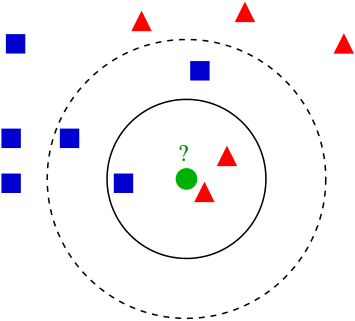
\includegraphics[width=0.7\linewidth]{img/knn_example}
	\caption{Esempio grafico dell'algoritmo KNN}
	\label{fig:knnexample}
\end{figure}


\subsection*{Scelta del parametro k}
La scelta del parametro dipende, ovviamente, dal tipo dei dati che abbiamo e dalla quantita', anche se in generale piu' e' grande $k$ meno rumore viene generato da questo algoritmo. Un buon metodo per trovare il giusto valore e' l'uso di tecniche euristiche, come la \textit{cross validation}. Un altra fonte di rumore di cui bisogna stare attenti e' la presenza di \textit{features} insignificanti nella ricerca del vicino. Per porre rimedio possiamo, ad esempio, usare un algoritmo genetico per selezionare le \textit{features} piu' significative

\subsection*{Cross validation}
Tecnica per migliorare le performance di un classificatore, consiste nel suddividere l'intero \textit{dataset} in $n$ parti uguali (di solito 10), ognuna delle quali svolgera' per una volta il ruolo di \textit{validation set} mentre il resto sara' il \textit{training set}. Questa tecnica risolve vari problemi tra i quali l'\textit{overfitting}.\\

\newpage
\section*{Naive bayes}
\subsection*{Teorema di bayes}
Un altro tipo di apprendimento usato per classificare le \textit{label} e' Naive bayes: esso si fonda sul famoso teorema di bayes enunciato come segue:
\begin{center}
	$P(B|A) = \dfrac{P(A|B)P(B)}{P(A)}$
\end{center}
Prima di spiegare in cosa consiste esattamente \textit{Naive Bayes}, occorre spiegare alcuni preconcetti:
\subsection*{Rete bayesiana}
Una rete bayesiana e' un grafo diretto aciclico i cui nodi rappresentano le variabili casuali del sistema analizzato mentre gli archi rappresentato la condizione di dipendenza fra nodi.
\begin{figure}[h]
	\centering
	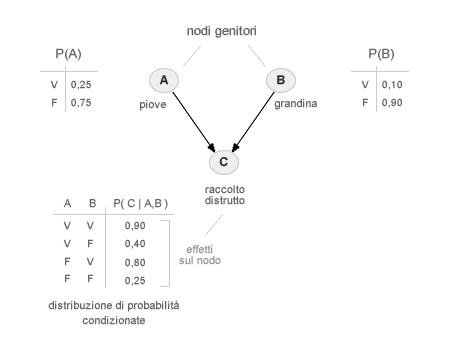
\includegraphics[width=0.7\linewidth]{img/rete-bayesiana-grafo.png}
	\caption{Esempio di rete bayesiana}
	\label{fig:rete-bayesiana-grafo}
\end{figure}





